% tQuant Architecture: technical description of the library (market data, class architecture, numerics,
% conventions). Filled in during the guided review, together with the notebooks.
% Build: latexmk (see .latexmkrc). Shared preamble: preamble.tex.
\documentclass[11pt,a4paper]{article}

% Shared preamble of the study documents (exercises.tex, models_and_pricing.tex, architecture.tex).
\usepackage[utf8]{inputenc}
\usepackage[T1]{fontenc}
\usepackage[english]{babel}
\usepackage{lmodern}
\usepackage[margin=2.5cm]{geometry}
\usepackage{amsmath,amssymb,amsthm,bm}
\usepackage{xcolor}
\usepackage[most]{tcolorbox}
\usetikzlibrary{arrows.meta,positioning,calc}
\usepackage{enumitem}
\usepackage{environ}
\usepackage{booktabs}
\usepackage{array}
\newcolumntype{L}[1]{>{\raggedright\arraybackslash}p{#1}}   % wrapped left-aligned column
\usepackage[skip=0.6\baselineskip plus 2pt, indent=0pt]{parskip}   % space between paragraphs, no indent
\usepackage{titlesec}
\titlespacing*{\section}{0pt}{5ex plus 1.5ex minus .5ex}{3ex plus .5ex}
\titlespacing*{\subsection}{0pt}{4ex plus 1ex minus .5ex}{2ex plus .3ex}
\titlespacing*{\paragraph}{0pt}{2.5ex plus .8ex minus .3ex}{1em}
\linespread{1.06}
\usepackage{etoolbox}
\pretocmd{\section}{\clearpage}{}{}   % every chapter (\section) starts on a new page
\pretocmd{\tableofcontents}{\begingroup\let\clearpage\relax}{}{}   % ... but the contents stay under the title
\apptocmd{\tableofcontents}{\endgroup}{}{}
\AtBeginDocument{%
  \setlength{\abovedisplayskip}{12pt plus 3pt minus 3pt}%
  \setlength{\belowdisplayskip}{12pt plus 3pt minus 3pt}%
  \setlength{\abovedisplayshortskip}{8pt plus 3pt}%
  \setlength{\belowdisplayshortskip}{8pt plus 3pt minus 2pt}}
\setlist{topsep=4pt, itemsep=2pt}   % lists: a little air (nosep still available)
\usepackage{hyperref}

\hypersetup{colorlinks=true, linkcolor=blue!50!black, urlcolor=blue!50!black}
\setlength{\emergencystretch}{3em}   % long \code{...} names: stretch lines instead of overfull boxes

% ── Math macros ─────────────────────────────────────────────────────────────
\newcommand{\E}{\mathbb{E}}
\newcommand{\Q}{\mathbb{Q}}
\newcommand{\R}{\mathbb{R}}
\newcommand{\dd}{\,\mathrm{d}}
\newcommand{\Nc}{\mathcal{N}}

% ── Cross references ────────────────────────────────────────────────────────
% Reference to a notebook in study/notebooks
\newcommand{\nb}[1]{\textsf{\small[notebook: \texttt{#1}]}}
% Reference to library code (module / class)
\newcommand{\code}[1]{\texttt{#1}}
% Section still to be written in the guided review
\newcommand{\pending}{\textcolor{gray}{\small\textit{To be written in the guided review.}}}


\title{tQuant --- Architecture}
\author{Andrea Carapelli}
\date{\today}

\begin{document}
\maketitle
\tableofcontents
\clearpage

\section*{Scope}
How the library is built: the market data (storage, keys, risk factors), the class architecture
(products, pricers, models, calibration), the numerical conventions (TensorFlow graphs, float64, AAD) and
the testing approach. The financial content of the models is in \emph{tQuant --- Models and Pricing}.

\section{Overview}\label{sec:arch-overview}

% ─────────────────────────────────────────────────────────────────────────────
\subsection{Design principles}\label{sec:arch-principles}
Prices as TensorFlow graphs, greeks by AAD, risk factors as float64 variables in the market objects,
one access point to market data.

\pending

% ─────────────────────────────────────────────────────────────────────────────
\subsection{Package layout}\label{sec:arch-layout}
\code{timehandles}, \code{numericalhandles}, \code{markethandles}, \code{index}, \code{flows},
\code{instruments}, \code{models}, \code{pricers}, \code{analytics}, \code{calibration}
(Figure~\ref{fig:arch-layout}).

% Package layout: how the modules connect, from the market data to prices and greeks.
\begin{figure}[ht]
\centering
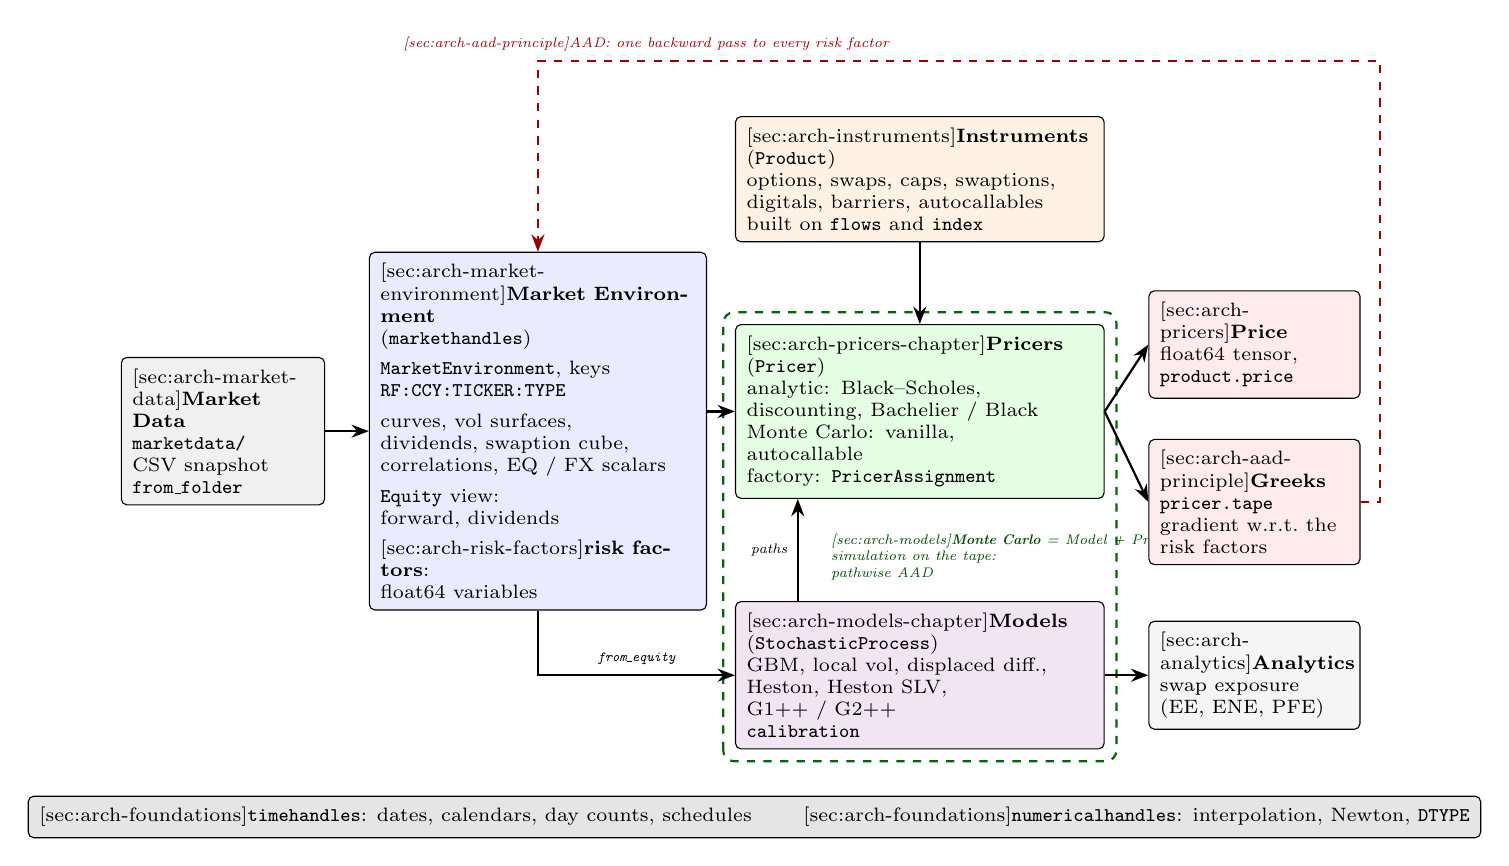
\begin{tikzpicture}[
    font=\scriptsize,
    >={Stealth[length=2.2mm]},
    box/.style={draw, rounded corners=2pt, align=left, inner sep=4pt, fill=#1},
    box/.default=white,
    flow/.style={->, thick},
    note/.style={font=\tiny\itshape, align=center},
  ]
  % ── data ──
  \node[box=gray!12, text width=2.3cm] (snap) at (-0.1, 0)
    {\hyperref[sec:arch-market-data]{\textbf{Market Data}}\\ \code{marketdata/}\\ CSV snapshot\\ \code{from\_folder}};

  % ── market ──
  \node[box=blue!8, text width=4.0cm] (mkt) at (3.9, 0)
    {\hyperref[sec:arch-market-environment]{\textbf{Market Environment}}\\ (\code{markethandles})\\[3pt]
     \code{MarketEnvironment}, keys\\ \code{RF:CCY:TICKER:TYPE}\\[3pt]
     curves, vol surfaces,\\ dividends, swaption cube,\\ correlations, EQ / FX scalars\\[3pt]
     \code{Equity} view:\\ forward, dividends\\[3pt]
     \hyperref[sec:arch-risk-factors]{\textbf{risk factors}}:\\ float64 variables};

  % ── products, pricers, models ──
  \node[box=orange!10, text width=4.4cm] (prod) at (8.75, 3.2)
    {\hyperref[sec:arch-instruments]{\textbf{Instruments}} (\code{Product})\\
     options, swaps, caps, swaptions,\\ digitals, barriers, autocallables\\
     built on \code{flows} and \code{index}};
  \node[box=green!10, text width=4.4cm] (pricer) at (8.75, 0.25)
    {\hyperref[sec:arch-pricers-chapter]{\textbf{Pricers}} (\code{Pricer})\\
     analytic: Black--Scholes,\\ discounting, Bachelier / Black\\
     Monte Carlo: vanilla,\\ autocallable\\
     factory: \code{PricerAssignment}};
  \node[box=violet!10, text width=4.4cm] (model) at (8.75, -3.1)
    {\hyperref[sec:arch-models-chapter]{\textbf{Models}} (\code{StochasticProcess})\\
     GBM, local vol, displaced diff.,\\ Heston, Heston SLV,\\ G1++ / G2++\\
     \code{calibration}};

  % Monte Carlo: model + pricer on the same tape
  \draw[dashed, thick, green!40!black, rounded corners=4pt]
    ($(model.south west) + (-0.15, -0.15)$) rectangle ($(pricer.north east) + (0.15, 0.15)$);
  \node[note, text=green!30!black, anchor=west, align=left] at (7.5, -1.6)
    {\hyperref[sec:arch-models]{\textbf{Monte Carlo}} = Model + Pricer\\ simulation on the tape:\\ pathwise AAD};

  % ── results ──
  \node[box=red!8, text width=2.4cm] (price) at (13.0, 1.1)
    {\hyperref[sec:arch-pricers]{\textbf{Price}}\\ float64 tensor,\\ \code{product.price}};
  \node[box=red!8, text width=2.4cm] (greeks) at (13.0, -0.9)
    {\hyperref[sec:arch-aad-principle]{\textbf{Greeks}}\\ \code{pricer.tape}\\ gradient w.r.t.\ the\\ risk factors};
  \node[box=gray!8, text width=2.4cm] (analytics) at (13.0, -3.1)
    {\hyperref[sec:arch-analytics]{\textbf{Analytics}}\\ swap exposure\\ (EE, ENE, PFE)};

  % ── foundations ──
  \node[box=gray!20, minimum width=15.3cm, align=center] (base) at (6.65, -4.9)
    {\hyperref[sec:arch-foundations]{\code{timehandles}}: dates, calendars, day counts, schedules \qquad
     \hyperref[sec:arch-foundations]{\code{numericalhandles}}: interpolation, Newton, \code{DTYPE}};

  % ── arrows ──
  \draw[flow] (snap.east) -- (snap.east -| mkt.west);
  \draw[flow] (mkt.east |- pricer.west) -- (pricer.west);
  \draw[flow] (mkt.south) |- node[pos=0.75, above, note] {\code{from\_equity}} (model.west);
  \draw[flow] (prod.south) -- (pricer.north);
  \draw[flow] (model.north -| 7.2, 0) -- node[left, note] {paths} (pricer.south -| 7.2, 0);
  \draw[flow] (pricer.east) -- (price.west);
  \draw[flow] (pricer.east) -- (greeks.west);
  \draw[flow] (model.east) -- (analytics.west);
  \draw[->, thick, dashed, red!60!black]
    (greeks.east) -- ++(0.25, 0) |- (6.65, 4.7) -| (mkt.north)
    node[pos=0.25, above, note] {\hyperref[sec:arch-aad-principle]{AAD: one backward pass to every risk factor}};
\end{tikzpicture}
\caption{Package layout. Market data enter only through the Market Environment, whose objects hold the risk factors as
float64 variables. A pricer turns an instrument and the market into a price graph: in closed form, or (Monte Carlo) by
simulating a model built from the same market variables, so the simulated paths are part of the graph. Either way the
gradient tape gives the greeks w.r.t.\ every risk factor in one backward pass. Dates, calendars, interpolation and solvers
sit underneath every package.}
\label{fig:arch-layout}
\end{figure}


% ─────────────────────────────────────────────────────────────────────────────
\subsection{Automatic differentiation}\label{sec:arch-aad-principle}
\paragraph{Reverse mode.} A price is a composition of elementary operations $v_k = \phi_k(v_{j}, j \prec k)$ from the
inputs $x$ (the risk factors) to the output $y$. The \emph{forward pass} evaluates them and records each operation with
the values it needs for its local derivatives (the \emph{tape}). The \emph{backward pass} walks the tape in reverse and
propagates the adjoints $\bar v_j = \partial y/\partial v_j$, starting from $\bar y = 1$:
\[
  \bar v_j = \sum_{k:\, j \prec k} \bar v_k\,\frac{\partial \phi_k}{\partial v_j},
  \qquad \frac{\partial y}{\partial x_i} = \bar x_i .
\]
One backward pass gives the gradient w.r.t.\ \emph{all} inputs, at a cost of a small multiple of the forward pass (2--5
in practice), whatever their number; bump-and-reprice needs one or two repricings per input. The price is memory: the
tape keeps the intermediate values (for a Monte Carlo price, of the order of paths $\times$ steps $\times$ state). Forward
mode (one directional derivative per pass) is the opposite trade-off, fit for few inputs and many outputs. The result is
the exact derivative of the computed function (up to rounding), not an approximation: where the code has a kink or a
jump, AAD differentiates the code as written.

\paragraph{TensorFlow.} The tape is \code{tf.GradientTape}: it records the operations on the watched tensors, and the
trainable variables (\code{tf.Variable}) are watched automatically. The call \code{tape.gradient(target, sources)} runs
the backward pass and returns the gradients with the structure of \code{sources} (a dict of lists, as \code{market\_env.risk\_factors()}). Mechanics that matter in the library:
\begin{itemize}[nosep]
  \item a tape is released after one \code{gradient} call (\code{persistent=True} for several); a tape inside another
        gives second derivatives (gamma); \code{tape.jacobian} gives the full Jacobian (calibration residuals);
  \item a source not connected to the target gets \code{None}, not 0: a value passed through \code{.numpy()},
        \code{float()}, a comparison or a cast to an integer leaves the graph;
  \item \code{tf.gather} on a variable returns sparse \code{IndexedSlices}: gathers are written to give dense gradients;
  \item \code{tf.stop\_gradient(v)} keeps the value and cuts the derivative;
  \item \code{tf.function} compiles the Python code into a graph, traced once per input signature and differentiable
        like eager code; the first call pays the tracing.
\end{itemize}

\paragraph{In tQuant.} Every market input is a float64 \code{tf.Variable} with a stable identity in the market objects
(bumps by \code{assign}), so a gradient w.r.t.\ \code{market\_env.risk\_factors()} is the full bucketed risk.
\code{Pricer.price(..., autodiff=True)} runs \code{calculate\_price} under a tape and keeps it on \code{pricer.tape};
pricers read the market only through its objects and never detach values. Patterns:
\begin{itemize}[nosep]
  \item \emph{Locating, not differentiating}: interval searches (interpolation, vol nodes, kernel bins) act on
        \code{stop\_gradient} copies; the derivative flows through the interpolation weights.
  \item \emph{Risk conventions}: a quantity deliberately held fixed is wrapped in \code{stop\_gradient} (the sticky
        implied yield of the continuous dividend model, the Heston parameters and $\E[v \mid X]$ in Heston SLV).
  \item \emph{Through a calibration}: the optimiser's iterations are not differentiated. At the optimum $\theta^*$ the
        implicit function theorem gives $\partial\theta/\partial m = -H^{-1}\,\partial^2 L/\partial\theta\,\partial m$; it is injected
        with a value-preserving step $\theta = \theta^* - (s - \mathrm{stop\_gradient}(s))$, $s = H^{-1}\nabla_\theta L(\theta^*, m)$
        ($H$ held): the value is $\theta^*$, the derivative the implicit one (Heston, displaced diffusion).
  \item \emph{Monte Carlo}: the tape over the simulation gives the pathwise derivative of the estimator, valid for
        Lipschitz payoffs; indicators (digitals, barriers) have no pathwise derivative and are smoothed by a sigmoid,
        or replaced by a continuous probability (the Brownian bridge of a barrier). Diagnostics such as the standard error
        are computed on \code{stop\_gradient} values.
\end{itemize}
The tests check AAD against central finite differences, with common random numbers for Monte Carlo
(\S\ref{sec:arch-testing}).

\section{Market data}\label{sec:arch-market-data}

% ─────────────────────────────────────────────────────────────────────────────
\subsection{Snapshots on disk}\label{sec:arch-snapshots}
\code{marketdata/<yyyymmdd>/<calibration\_set>/} and its CSV files; the synthetic generator.

\pending

% ─────────────────────────────────────────────────────────────────────────────
\subsection{MarketEnvironment and keys}\label{sec:arch-market-env}
Keys \code{RISKFACTOR:CCY:TICKER:TYPE}, validation, typed accessors, I/O round trip.
\nb{01\_market\_handles.ipynb}

\pending

% ─────────────────────────────────────────────────────────────────────────────
\subsection{Market objects and risk factors}\label{sec:arch-risk-factors}
\code{RateCurve}, \code{VolatilitySurface}, \code{DividendCurve}, \code{SwaptionVolCube},
\code{CorrelationMatrix}, scalar equity data; \code{risk\_factors()}.

\pending

% ─────────────────────────────────────────────────────────────────────────────
\subsection{The Equity view}\label{sec:arch-equity}
References to spot, repo, dividends, surface and discount curve; single place for the forward.
\nb{03\_equity\_underlying.ipynb}

\pending

\section{Class architecture}\label{sec:arch-classes}

% ─────────────────────────────────────────────────────────────────────────────
\subsection{Products and cash flows}\label{sec:arch-products}
\code{Product} and the instruments; \code{flows/} coupons and legs; generators.

\pending

Equity options derive from \code{Option}, which holds the option type, the strike (a float64 variable), the
exercise type and the underlying. \code{VanillaOption} is European or American; \code{DigitalOption} is European, with a
\code{payoff\_type} (\code{CashOrNothing} or \code{AssetOrNothing}, enum \code{PayoffType}) and a \code{cash\_amount}.
\code{BlackScholesPricer} prices both, the digitals through \code{digital\_calc}; the factory maps a digital to it.
\code{VanillaMCPricer} prices both too; for the digital payoff \code{digital\_smoothing} sets the sigmoid width (default
1\% of the strike, 0 for the hard indicator). \nb{digital\_options.ipynb}

The barrier option class, \code{BarrierOption} in \code{instruments/barrier.py}, adds the level \code{barrier}, the
type \code{barrier\_type} (an enum \code{BarrierType} with the members \code{DownIn}, \code{DownOut}, \code{UpIn} and
\code{UpOut}, and the flags \code{is\_down} and \code{is\_in}) and the dates \code{monitoring\_dates}, where \code{None}
means continuous monitoring (property \code{continuous}). \code{BlackScholesPricer} prices it through \code{barrier\_calc}
(\code{pricers/black.py}); \code{VanillaMCPricer} through \code{\_bridge\_survival} (continuous) or
\code{\_discrete\_survival} (monitoring dates merged into the grid).

With the autocall at an unreachable level, an \code{AutocallableOption} is a strip of digitals (put barrier 0) or a
put knocked in at expiry (coupons 0).
\nb{digital\_strip.ipynb}, \nb{down\_and\_in\_put.ipynb}

% ─────────────────────────────────────────────────────────────────────────────
\subsection{Pricers}\label{sec:arch-pricers}
\code{Pricer}: \code{calculate\_price}, \code{price(..., autodiff)}, the tape; \code{PricerAssignment}.

A pricer implements \code{calculate\_price(product, market\_env)}: a TensorFlow graph from the market objects (read only
through the \code{MarketEnvironment} accessors, never copied or detached with \code{.numpy()}) to a float64 price.
\code{Pricer.price(product, market\_env, autodiff=False)} runs it, stores the price on \code{product.price} and, with
\code{autodiff=True}, keeps the \code{GradientTape} on \code{pricer.tape}: the greeks are
\code{pricer.tape.gradient(product.price, variables)} for any market variables (or all of them,
\code{market\_env.risk\_factors()}); a second tape around the call gives second orders (gamma). The only variable a
pricer may create is the time to maturity, left on the product (\code{product.time\_to\_maturity}) for theta.
\code{PricerAssignment.create(product)} picks the default pricer by \code{isinstance}: \code{VanillaOption}
$\to$ \code{BlackScholesPricer}, the rates products to their discounting / Bachelier pricers; Monte Carlo pricers are
chosen explicitly. \code{BlackScholesPricer(dividend\_model, use\_implied\_repo)}: European by the Black formula,
American by Bjerksund--Stensland (\code{pricers/black.py}), inputs from the \code{Equity} view, diagnostics on the
product (Market data, The Equity view). \nb{black\_scholes.ipynb}

% ─────────────────────────────────────────────────────────────────────────────
\subsection{Models}\label{sec:arch-models}
\code{StochasticProcess} (\code{size}, \code{initial\_values}, \code{noise\_size}, \code{evolve}) and the
\code{from\_equity} factories used by the Monte Carlo pricers.

\code{StochasticProcess} (\code{models/stochasticprocess.py}) is the common interface: \code{size()} (state
dimension), \code{initial\_values()}, \code{noise\_size()} (normals per path and step, default 1) and
\code{evolve(t\_grid, dw, observation\_times=None)}, which maps pre-drawn normals \code{dw}
($[n_{\text{paths}}, n_{\text{steps}}]$, or with a trailing axis of size \code{noise\_size()}) to paths on the increasing grid
\code{t\_grid} (no 0), returning only the \code{observation\_times} columns when given. The caller draws the normals
(\code{tf.random.stateless\_normal} with a seed), which makes the paths reproducible and the bumps common-random-number
ones. Equity models have a \code{from\_equity(equity, maturity, strike)} factory that builds them from the market
variables, so the simulation is differentiable w.r.t.\ them. They are the GBM (\code{GeometricBrownianMotion},
exact steps), local vol, displaced diffusion, Heston and Heston SLV.
\code{VanillaMCPricer(model, n\_paths, n\_steps, seed, digital\_smoothing)} takes the model \emph{class}, calls
\code{from\_equity} at each price, simulates on a uniform grid ending at the expiry and leaves
\code{standard\_error}, \code{discount\_factor} and \code{time\_to\_maturity} on the product. \nb{monte\_carlo\_gbm.ipynb}

% ─────────────────────────────────────────────────────────────────────────────
\subsection{Calibration}\label{sec:arch-calibration}
Calibration inside the factories (implicit-function greeks) and the rates calibration module.

\pending

\section{Numerics}\label{sec:arch-numerics}

% ─────────────────────────────────────────────────────────────────────────────
\subsection{Float64 and dtypes}\label{sec:arch-dtypes}
\code{DTYPE}, \code{as\_variable}, the float32 round trip of \code{tf.cast} on Python numbers.

\pending

% ─────────────────────────────────────────────────────────────────────────────
\subsection{AAD in practice}\label{sec:arch-aad}
\code{GradientTape}, dense gradients (no \code{IndexedSlices}), \code{tf.function} and loops,
\code{stop\_gradient} where a derivative must not flow.

\pending

% ─────────────────────────────────────────────────────────────────────────────
\subsection{Performance}\label{sec:arch-performance}
Compiled functions traced once, batching, vectorised closed forms.

\pending

\section{Testing}\label{sec:arch-testing}

% ─────────────────────────────────────────────────────────────────────────────
\subsection{Strategy}\label{sec:arch-test-strategy}
Unit tests as the regression check: pinned numbers, independent references (closed forms, parity, finite
differences vs AAD, Monte Carlo within standard errors), synthetic self-contained fixtures.

\pending


\end{document}
